\documentclass{article}%
\usepackage[T1]{fontenc}%
\usepackage[utf8]{inputenc}%
\usepackage{lmodern}%
\usepackage{textcomp}%
\usepackage{lastpage}%
\usepackage{authblk}%
\usepackage{graphicx}%
%
\title{Pathological Impact of Hepatitis B Virus Surface Proteins on the Liver Is Associated with the Host Genetic Background}%
\author{Dawn Silva}%
\affil{Nephrology Unit, Department of Medicine, Faculty of Medicine, Thammasat University (Rangsit Campus), Khlong Nueng, Khlong Luang, Pathum Thani 12121, Thailand}%
\date{01{-}01{-}2014}%
%
\begin{document}%
\normalsize%
\maketitle%
\section{Abstract}%
\label{sec:Abstract}%
TUESDAY, DEC 28, 2013 {-}{-} Dr. Christopher Cepharthine and his team at Cepharanthine are creating a novel compound that they believe could be used to regulate production of a critical molecule in mammalian cells. At first, this molecule, referred to as MDR1, is the pathway for the growth and survival of specific, critical regulatory functions in tissues. Now, Dr. Cepharthine and his team believe that this molecule has tremendous potential to regulate a wide range of cell functions and eventually be used in treating a wide range of diseases.\newline%
In my conversation with Dr. Cepharthine I asked him about one of the first discoveries he made in his lab. Two years ago I actually found a sequence in the human genome that was important for regulating prostate cancer cells, said Dr. Cepharthine. I also found that as prostate cancer spread, its cells grow much more quickly, and in turn produced more copies of a peptide molecule called DKK1 that controls how fast it grows.\newline%
Dr. Cepharthine explained that DKK1 is an interleukin 2 (IL{-}2) molecule that regulates the breakdown of a protein called prostate{-}specific antigen (PSA). It was the property of DKK1 that it normally has very little {-} and seemingly impossible to deal with {-} accumulation in the lungs. To my surprise, it wasnt getting into the lungs, and over the past year or so, weve been using DKK1 as the metabolic pathway that puts into which the plaque in the arteries were formed, and after the plaque formed, DKK1 rapidly leached out of the lungs. I think thats a surprising discovery, because at that time there were only two active genes in prostate{-}specific antigen that were associated with cancer, and these two gene didnt seem to have an effect.\newline%
His team soon discovered that the combination of these two genes involved with triggering prostate cancer production can cause prostate cancer cells to grow much faster, which in turn, leads to increased tumors. By obtaining a compound that activates DKK1, Dr. Cepharthine and his team are working on enhancing the efficacy of these inhibitors in mammals.\newline%
This is only the first discovery in that were trying to control the cascade at the molecular level to influence genes, and then to exert small but significant effects, said Dr. Cepharthine. It has potential to exert a deleterious impact in terms of sensitivity of growth and cancer cell proliferation in a broad array of organisms, from nervous system cells to lung cells to bone cells.\newline%
Dr. Cepharthine is working to develop further compound inhibitors to block this function in a wide range of animals and diseases, including:\newline%
 Chronic fatigue syndrome, in which increases tumor growth and subsequent recurrence of cancer,\newline%
 Cervical cancer, in which the female cancer cell metastasizes and also destroys the protective tissue surrounding her cervix,\newline%
 Herpes, which, similar to prostate cancer, increases the bodys immune response to the virus.\newline%
 DMPA2{-}A, a pro{-}statin receptor that disrupts the hearts function, allowing the heart to pump less blood.\newline%
 DMPA{-}2A has been shown to cause heart attacks and stroke in human animals and was removed from drug class one after it was linked to metabolic syndrome.\newline%
We know that human endothelial cells have proteins that are

%
\subsection{Image Analysis}%
\label{subsec:ImageAnalysis}%


\begin{figure}[h!]%
\centering%
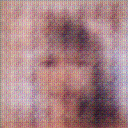
\includegraphics[width=150px]{500_fake_images/samples_5_379.png}%
\caption{A Close Up Of A Black And White Cat}%
\end{figure}

%
\end{document}